% !TeX program = pdflatex
\documentclass[tikz,border=8pt]{standalone}
\usepackage{tikz}
\definecolor{FigureBlue}{HTML}{2563EB}\definecolor{FigureOrange}{HTML}{EA580C}\definecolor{FigureGreen}{HTML}{16A34A}
\begin{document}
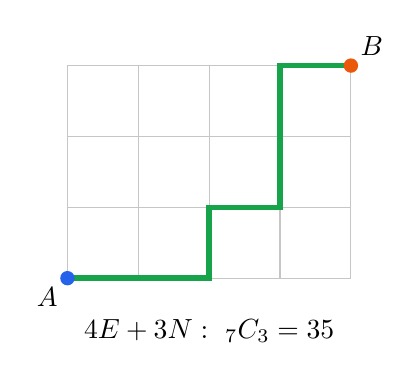
\begin{tikzpicture}[x=.9cm,y=.9cm]
  \draw[step=1,gray!45] (0,0) grid (4,3);
  \draw[FigureGreen,line width=2pt] (0,0)--(2,0)--(2,1)--(3,1)--(3,3)--(4,3);
  \fill[FigureBlue] (0,0) circle (2.6pt); \fill[FigureOrange] (4,3) circle (2.6pt);
  \node[below left] at (0,0) {$A$}; \node[above right] at (4,3) {$B$};
  \node at (2,-.75) {$4E+3N:\ {}_{7}C_{3}=35$};
\end{tikzpicture}
\end{document}
